\documentclass[11pt]{jsarticle}
\usepackage{amsmath,amssymb} % 数式を使うため
\usepackage{mathdots} % 数式内の右肩上がり3点 \iddots
\usepackage{bm} % ベクトルの太字 \bm{}
\usepackage{ascmac} % 枠で囲む環境 itembox, screen, boxnote, shadebox
\usepackage{booktabs} % 欧米風のテーブル環境 \tabular の中で \toprule,\midrule, \bottmrule
\usepackage{multirow} % テーブルの複数行に渡る項目 \multirow{行数}{*}{内容}
\usepackage[dvipdfmx,bookmarks=true,bookmarksnumbered=true]{hyperref} % PDF 文書内に URL へのリンクを貼る \url{アドレス}
\usepackage{pxjahyper} % 日本語のしおりを付けるため。hyperref と対で使用
\hypersetup{colorlinks=true,linkcolor=blue, citecolor=blue, urlcolor=blue} % リンクを下線からカラーリンクに変更。hyperref と対で使用
\usepackage{listings, jlisting} % ソースコードを書くため \begin{lslisting}\end{lslistiing}
\def\lstlistingname{ソースコード}
\lstset{%
	tabsize = 3, % タプインデントの大きさ
	basicstyle = \footnotesize, % 基本の文字スタイル
	keywordstyle = \bfseries\color{blue}, % キーワード
	stringstyle = \color{red}, % 文字列
	showstringspaces=false,
	commentstyle = \color[rgb]{0,0.5,0}, % コメント
	framesep = 10pt, % 
	xleftmargin = 20pt, % 左インデント
	xrightmargin = 20pt, % 右インデント
}
\lstdefinestyle{MATLABStyle}{%
	language = Matlab,
	frame=single, % フレームの書式
	backgroundcolor = {\color[gray]{0.96}}, % 背景色を灰色
	numbers = {left}, % 行番号の位置
	numberstyle = {\footnotesize}, % 行番号のスタイル
	numbersep = {2zw}, % コードから行番号までの距離
	morekeywords = {cout, cin, end}
}
\usepackage[hiresbb,dvipdfmx]{graphicx} % PDF, PNG, JPEG, EPS の画像を扱うため
\usepackage{wrapfig} % 図などを文章が回り込むように \begin{wrapfigure} \begin{wraptable}
\usepackage{makeidx} % 索引を作るため \makeindex と対に
\makeindex % 索引を作る:索引をおきたい場所に \printindex を置く

\newtheorem{theorem}{定理}[section]	% 定理環境の定義
\newtheorem{defi}{定義} 		% 定義環境の定義
\newtheorem{coro}{系}		% 系環境の定義
\newtheorem{lemm}{補題} 		% 補題環境の定義

\newcommand{\ten}[1]{{{}^t #1}} % 行列ベクトルの転置 tA を書くため \ten{A}
\renewcommand{\vec}[1]{\bm{#1}} % \bm{x} の代わりに \vec{x}

\newcommand{\inpro}[2]{{\vec{#1}^t\vec{#2}}}

\newenvironment{pocketList}{
   \begin{center}
   \begin{tabular}{ccc} \toprule
   名前 & 分類 & 特性 \\ \midrule
}{
   \\ \bottomrule
   \end{tabular}
   \end{center}
}

\setcounter{tocdepth}{3} % subsubsection まで目次に載せる=3, subsection=2, section=1

%%%%%%%%%%%%%%%%%%%%%%%%%%%%%%%%%%%%%%%%%%%%%%%%%%%%%%%%%%%%%%%%%%
\begin{document}


%1.実験に見合ったタイトル, 学籍番号, 氏名, 日付などを記した表紙をつける
\title{数値解析学}
\author{Sumire}
\date{2022.12.22}
\maketitle

%表紙にメモ(概要)
\begin{abstract}
\centerline{常微分方程式の数値解析}
\end{abstract}

\clearpage
%目次
\tableofcontents

\clearpage
%表目次
\listoftables
%図目次
\listoffigures

\clearpage
%%%%%%%%%%%%%%%%%%%%%%%%%%%%%%%%%%%%%%%%%%%%%%%%%%%%%%%%%%%%%%%%%%
%2.実験目的(実験を行う動機や背景となった問題点などを述べて目的を明確にする)
\section{実験目的}
また, report 1 のときには深く考える余裕はなかったが, 微分方程式がどのように応用されているのかを知り, 数理モデル化するなど理解さらにを深めたいと思った。



%%%%%%%%%%%%%%%%%%%%%%%%%%%%%%%%%%%%%%%%%%%%%%%%%%%%%%%%%%%%%%%%%%%%%%%%%%%%%%%%%%%%%%%%%%%%%%%%%%%%%%%
%3.問題設定(扱う方程式や解法,パラメータの設定など)
\section{問題設定}
今回は, 課題 II を扱う. \\
van der Pol 方程式
\[
\left\{
\begin{array}{l}
\displaystyle \frac{d^{2}x}{dt^{2}} - \mu (1 - x^{2})\frac{dx}{dt} + \omega^{2}x = 0 \ \ \ \ \ 0 < t < T, \\
\ \\
\displaystyle x(0) = x_{0} ,\ \ \frac{dx}{dt}(0) = y_{0}
\end{array}
\right.
\]

に対して, Euler法とHeun法を適用し, 初期値とパラメータ$(\mu, \omega)$ によって回の振る舞い, 解の精度, 収束の速さを, 以下を例に調べよ. 
\ \\
\begin{itemize}
\item[1.] 解の様子をグラフで表示する. 
	\begin{itemize}
	\item[(a)] $\displaystyle y = \frac{dx}{dt}$ とする. $\omega = 1$, $\mu = 1$, $(x_{0}, y_{0}) = (-4, 3)$, $T = 15$, $N = 1500$ に対して, $(t, x(t))$, $(t, y(t))$, $(x(t)t, y(t))$ の散布図を描いてみる. 
	\item[(b)] 初期値$(x_{0},y_{0})$とパラメータ$(\mu,\omega)$を変えて,解の様子を調べてみる.
	\end{itemize}
\ \\
\item[2.] 数値解の誤差と収束の速さを考察する. \\
	$\omega = 1$, $\mu = 1$, $(x_{0}, y_{0}) = (-4, -3)$, $T = 4$ と固定する. $N$ を十分大きく取ったとき(例: $N = 10000$), Heun法によって得られた近似解 $x_{10000} =: x_{s}$ を真の解と見なし, 以下の考察をする.
	\begin{itemize}
	\item[(a)] $N = 100, 200, 400, 800, 1600$ に対して, Euler法によって得られた近似解 $x^{Euler}_{N}$ と $x_{s}$ の誤差 $|x^{Euler}_{N} - x_{s}|$ を計算し, 誤差と刻み幅 $h = T/N$ の関係を調べ, 収束の速さを考察する.
	\item[(b)] $N = 100, 200, 400, 800, 1600$ に対して, Heun法によって得られた近似解 $x^{Heun}_{N}$ と $x_{s}$ の誤差 $|x^{Heun}_{N} - x_{s}|$ を計算し, 誤差と刻み幅 $h = T/N$ の関係を調べ, 収束の速さを考察する.
	\end{itemize}
\end{itemize}



%%%%%%%%%%%%%%%%%%%%%%%%%%%%%%%%%%%%%%%%%%%%%%%%%%%%%%%%%%%%%%%%%%%%%%%%%%%%%%%%%%%%%%%%%%%%%%%%%%%%%%%
% 4.理論(分かっている理論的な事実や解析結果,また自身の予想など)
\section{理論}
まず初めに, わかっている理論的な事実について述べる. \\
常微分方程式とは, 未知数とその導関数含み, 独立変数が1つの方程式のことを言う. \\
van der Pol 方程式は, 2階微分方程式である. van der Pol 方程式を支配方程式とするのが, van der Pol 振動子である. (支配方程式とは, 物理現象の数理モデルを構築するために, その現象を数学的に方程式で表したものを指す. ) \\
van der Pol 方程式を一般化した方程式に, Li\'{e}nard の方程式というものがある. \\

\begin{itembox}[c]{Li\'{e}nard の定理}
Li\'{e}nard の方程式 \\
\[ \begin{pmatrix} \displaystyle \frac{dx_1}{dt} \\ \displaystyle \frac{dx_2}{dt} \end{pmatrix} = \begin{pmatrix} \displaystyle x_2 \\ \displaystyle -f(x_1)x_2 - g(x_1) \end{pmatrix}\]
について, 
\begin{itemize}
\item[1.] $f$, $g$ が連続微分可能
\item[2.] $g$ は奇関数
\item[3.] $x > 0$ のとき, $g(x) > 0$
\item[4.] $f$ は偶関数
\item[5.] $F(x) := \int_{0}^{x} f(s) ds$ と置く. \\
$F(a) = 0$, $0 < x < a$ ならば, $F(x) < 0$, $x > a$ ならば $F(x) > 0$ で広義単調増加で $\lim_{x \to \infty} F(x) = \infty$. これ満たす $a > 0$ が存在する. 
\end{itemize}
これらの条件を満たすとき, 方程式はただひとつの漸近安定なリミットサイクルが存在する. 
\end{itembox}
リミットサイクルとは, 力学系における位相空間上での閉軌道のことである. \\
\ \\
Van der Pol方程式は支配方程式が非線形の摩擦項を持つ2階微分方程式で記述される. 摩擦項は, ある決まった範囲にある場合(範囲は摩擦項の係数によって変化する)は正の摩擦となる. つまり, 振動を減衰させる方向に作
用する. しかしそのの範囲外では, 負の摩擦となり, 振動を成長させる方向に作用する. (減衰力は負
となる. )減衰振動と発散振動の境界(リミットサイクル)が存在していることになる. 
\ \\
\ \\
それでは, 課題IIの方程式を見ていく. \\
$\displaystyle y = \frac{dx}{dt}$ とおくと, 課題IIの方程式は, 
\[
\left\{
\begin{array}{l}
\displaystyle \frac{dy}{dt} - \mu (1 - x^{2}) y + \omega^{2}x = 0 \ \ \ \ \ 0 < t < T, \\
\ \\
\displaystyle \frac{dx}{dt} = y\ \ \ \ \ \ \ \ \ \ \ \ \ \ \ \ \ \ \ \ \ \ \ \ \ \ \ \ \ \ \ 0 < t < T, \\
\ \\
\displaystyle x(0) = x_{0} ,\ \ y(0) = y_{0}
\end{array}
\right.
\]

と変形できる. \\
今回は, Van der Pol 方程式を変形したあとの方程式に対して, Euler法, Heun法を適用していく. 


\clearpage
%%%%%%%%%%%%%%%%%%%%%%%%%%%%%%%%%%%%%%%%%%%%%%%%%%%%%%%%%%%%%%%%%%%%%%%%%%%%%%%%%%%%%%%%%%%%%%%%%%%%%%%
%5.実験結果(表やグラフなどを利用して見やすくする)
% 青:Euler
% 赤:Heun
\section{実験結果}
%1.a %%%%%%%%%%%%%%%%%%%%%%%%%%%%%%%%%%%%%%%%%%%%%%
\subsection{1. 解の様子をグラフで表示する. }

%1.a %%%%%%%%%%%%%%%%%%%%%%%%%%%%%%%%%%%%%%%%%%%%%%
\subsubsection{}
\begin{itembox}[l]{1. (a)}
$\displaystyle y = \frac{dx}{dt}$ とする. $\omega = 1$, $\mu = 1$, $(x_{0}, y_{0}) = (-4, 3)$, $T = 15$, $N = 1500$ に対して, $(t, x(t))$, $(t, y(t))$, $(x(t)t, y(t))$ の散布図を描いてみる. 
\end{itembox}

$\displaystyle y = \frac{dx}{dy}$ とし, $\omega = 1$, $\mu = 1$, $(x_{0}, y_{0}) = (-4, 3)$ とすると, van der Pol 方程式は, 
\[
\left\{
\begin{array}{l}
\displaystyle \frac{dy}{dt} - (1 - x^{2})y + x = 0 \ \ \ \ \ 0 < t < T, \\
\ \\
\displaystyle \frac{dx}{dt} = y\ \ \ \ \ \ \ \ \ \ \ \ \ \ \ \ \ \ \ \ \ \ \ \ \ \ 0 < t < T, \\
\ \\
\displaystyle x(0) = -4 ,\ \ y(0) = -3
\end{array}
\right.
\]
となる. 

$T = 15$, $N = 1500$ に対する, $(t, x(t))$, $(t, y(t))$, $(x(t)t, y(t))$ の散布図は以下のようである. 
\begin{figure}[htbp]
\centering
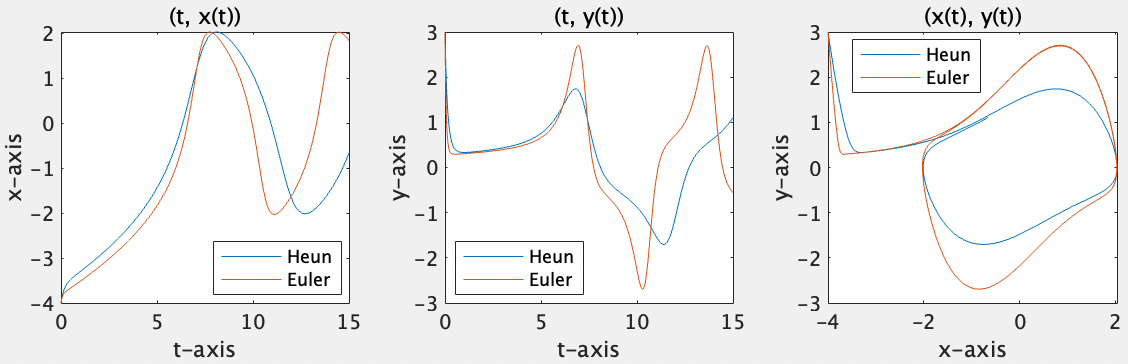
\includegraphics[width=15cm]{images/1_a_1*.png}
\caption{$\omega = 1$, $\mu = 1$, $(x_{0}, y_{0}) = (-4, 3)$, $T = 15$, $N = 1500$}
\end{figure}

%1.b %%%%%%%%%%%%%%%%%%%%%%%%%%%%%%%%%%%%%%%%%%%%%%
\subsubsection{}
\begin{itembox}[l]{1. (b)}
初期値$(x_{0},y_{0})$とパラメータ$(\mu,\omega)$を変えて,解の様子を調べてみる. 
\end{itembox}

まず初めに, $T = 15$, $N = 1500$, パラメータ $\mu = 1$, $\omega = 1$ と固定して, 初期値 $(x_{0}, y_{0})$ を変えて実験を行う. 今回は, 初期値の符号に着目する. 

\begin{figure}[htbp]
\centering
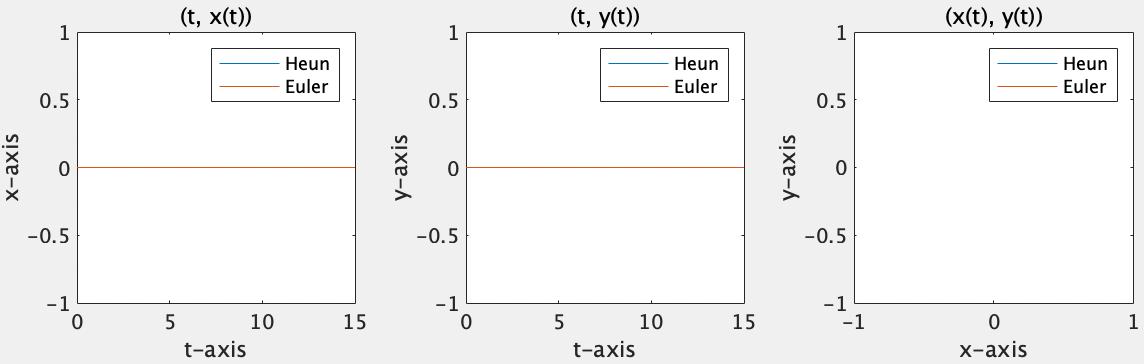
\includegraphics[width=9cm]{images/1_b_1_zero*.png}
\caption{$(x_{0}, y_{0}) = (0, 0)$}
\end{figure}

\begin{figure}[htbp]
\centering
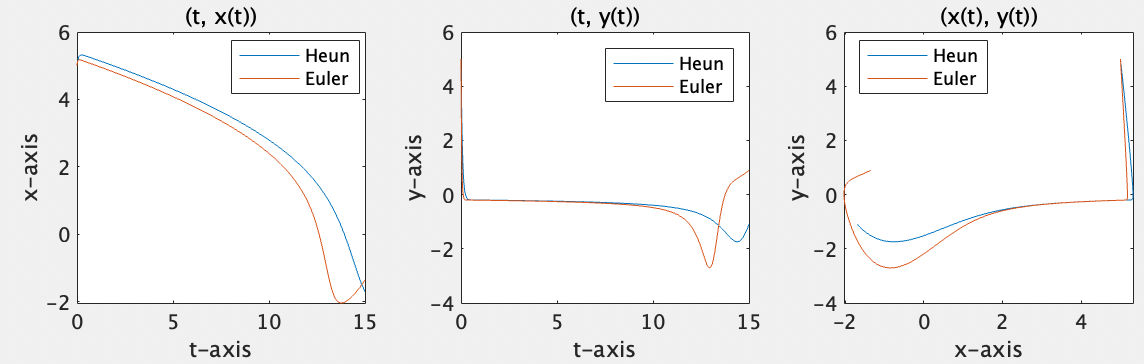
\includegraphics[width=9cm]{images/1_b_1_pp*.png}
\caption{$(x_{0}, y_{0}) = (5, 5)$ }
\end{figure}

\begin{figure}[htbp]
\centering
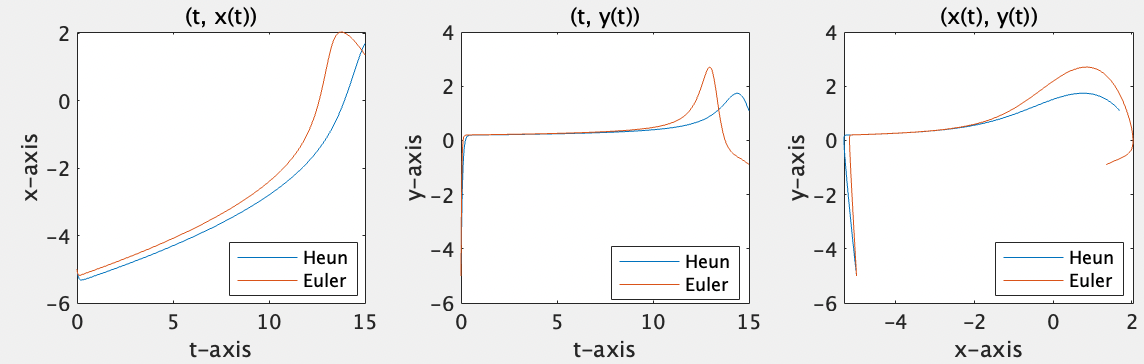
\includegraphics[width=9cm]{images/1_b_1_nn*.png}
\caption{$(x_{0}, y_{0}) = (-5, -5)$}
\end{figure}

\begin{figure}[htbp]
\centering
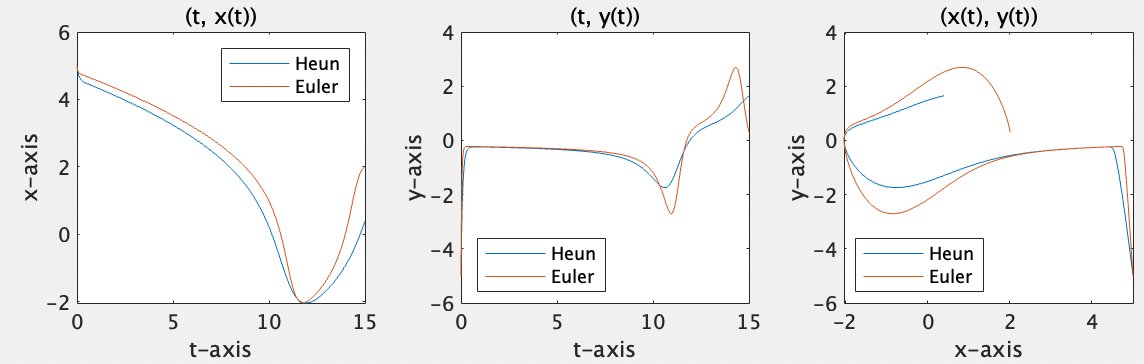
\includegraphics[width=9cm]{images/1_b_1_pn*.png}
\caption{$(x_{0}, y_{0}) = (5, -5)$}
\end{figure}

\begin{figure}[htbp]
\centering
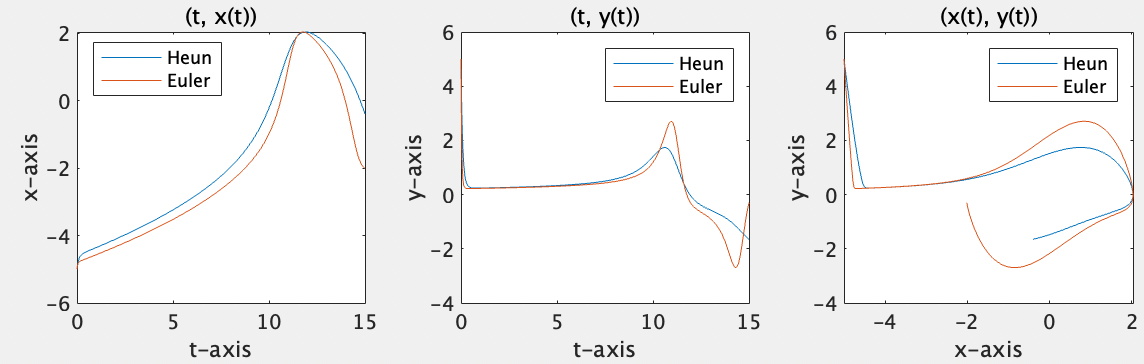
\includegraphics[width=9cm]{images/1_b_1_np*.png}
\caption{$(x_{0}, y_{0}) = (-5, 5)$}
\end{figure}
\ \\
次に, $T = 15$, $N = 1500$, 初期値 $(x_{0}, y_{0}) = (5, -5)$ と固定して, パラメータ $\mu$, $\omega$ を変えて実験を行う. ここでは, パラメータの符号に着目する. ($\omega$ は方程式において二乗されているため, 絶対値を考える. )

\begin{figure}[htbp]
\centering
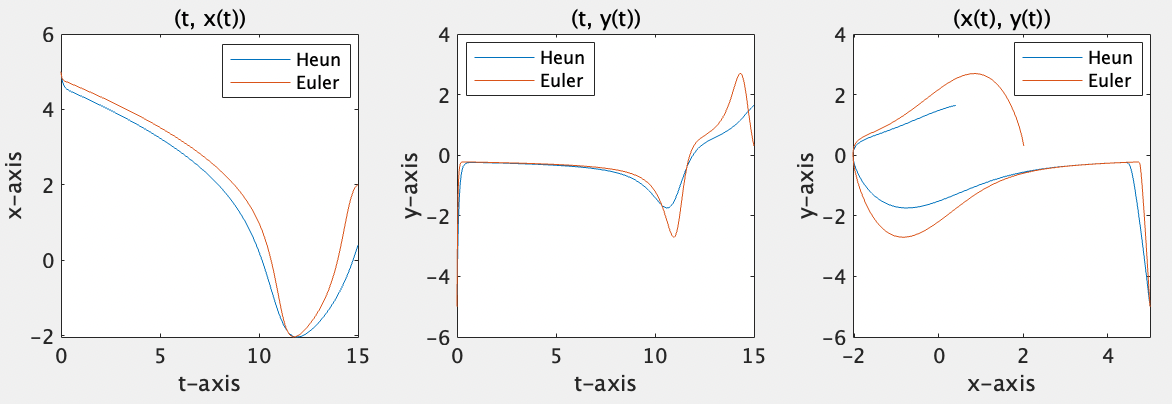
\includegraphics[width=9cm]{images/1_b_2_iti*.png}
\caption{$\mu = 1$, $|\omega| = 1$}
\end{figure}

\begin{figure}[htbp]
\centering
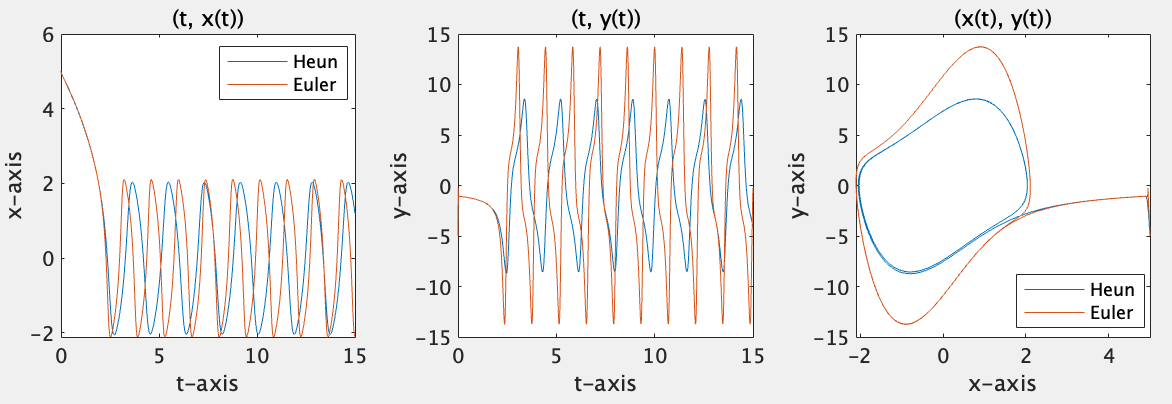
\includegraphics[width=9cm]{images/1_b_2_pp*.png}
\caption{$\mu = 5$, $|\omega| = 5$}
\end{figure}

\begin{figure}[htbp]
\centering
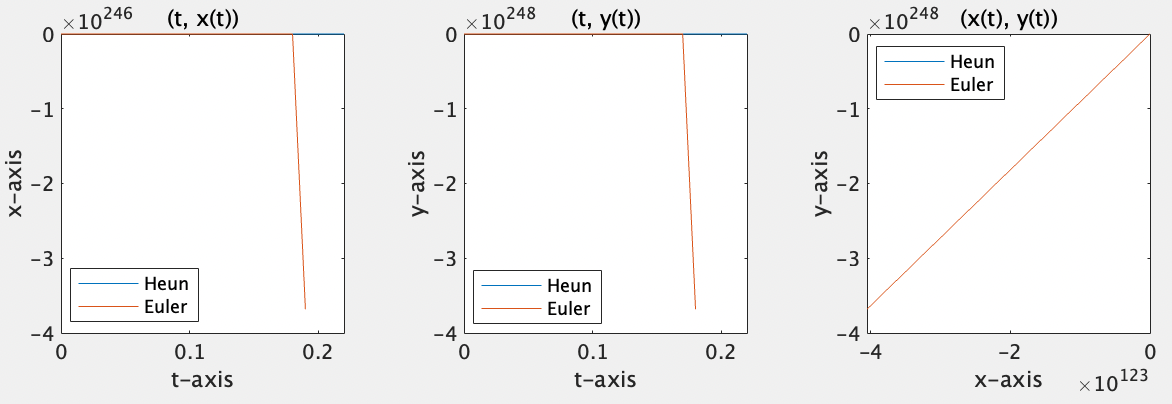
\includegraphics[width=9cm]{images/1_b_2_nn*.png}
\caption{$\mu = -5$, $|\omega| = 5$}
\end{figure}

%2. %%%%%%%%%%%%%%%%%%%%%%%%%%%%%%%%%%%%%%%%%%%%%%
\subsection{2. 数値解の誤差と収束の速さを考察する. }
$\omega = 1$, $\mu = 1$, $(x_{0}, y_{0}) = (-4, -3)$, $T = 4$ と固定する. $N$ を十分大きく取ったとき(例: $N = 10000$), Heun法によって得られた近似解 $x_{10000} =: x_{s}$ を真の解と見なし, 以下の考察をする. \\
以下, $x_{10000} =: x_{s} = -3.287011966884707e+00$ を用いる. 

%2.a %%%%%%%%%%%%%%%%%%%%%%%%%%%%%%%%%%%%%%%%%%%%%%
\subsubsection{}
\begin{itembox}[l]{2. (a)}
$N = 100, 200, 400, 800, 1600$ に対して, Euler法によって得られた近似解 $x^{Euler}_{N}$ と $x_{s}$ の誤差 $|x^{Euler}_{N} - x_{s}|$ を計算し, 誤差と刻み幅 $h = T/N$ の関係を調べ, 収束の速さを考察する. 
\end{itembox}

\begin{table}[htbp]
\centering
\begin{tabular}{|c||c|c|} \hline
\textbf{$N$} & \textbf{$x^{Euler}_{N}$} & \textbf{$|x^{Euler}_{N}-x_{s}|$} \\ \hline
$100$ & $-3.0235e+00$ & $2.6351e-01$ \\ \hline
$200$ & $-3.0187e+00$ & $2.6834e-01$ \\ \hline
$400$ & $-3.0168e+00$ & $2.7023e-01$ \\ \hline
$800$ & $-3.0159e+00$ & $ 2.7108e-01$ \\ \hline
$1600$ & $-3.0155e+00$ & $2.7148e-01$ \\ \hline
\end{tabular}
\caption{$|x^{Euler}_{N}-x_{s}|$}
\end{table}

%2.b %%%%%%%%%%%%%%%%%%%%%%%%%%%%%%%%%%%%%%%%%%%%%%
\subsubsection{}
\begin{itembox}[l]{2. (b)}
$N = 100, 200, 400, 800, 1600$ に対して, Heun法によって得られた近似解 $x^{Heun}_{N}$ と $x_{s}$ の誤差 $|x^{Heun}_{N} - x_{s}|$ を計算し, 誤差と刻み幅 $h = T/N$ の関係を調べ, 収束の速さを考察する.
\end{itembox}

\begin{table}[htbp]
\centering
\begin{tabular}{|c||c|c|} \hline
\textbf{$N$} & \textbf{$x^{Heun}_{N}$} & \textbf{$|x^{Heun}_{N}-x_{s}|$} \\ \hline
$100$ & $-3.2135e+00$ & $7.3471e-02$ \\ \hline
$200$ & $-3.2507e+00$ & $3.6312e-02$ \\ \hline
$400$ & $-3.2692e+00$ & $1.7773e-02$ \\ \hline
$800$ & $-3.2785e+00$ & $8.5129e-03$ \\ \hline
$1600$ & $-3.2831e+00$ & $3.8856e-03$ \\ \hline
\end{tabular}
\caption{$|x^{Heun}_{N}-x_{s}|$}
\end{table}



\clearpage
%%%%%%%%%%%%%%%%%%%%%%%%%%%%%%%%%%%%%%%%%%%%%%%%%%%%%%%%%%%%%%%%%%%%%%%%%%%%%%%%%%%%%%%%%%%%%%%%%%%%%%%
%6.考察(理論的・数値的な側面からできる限り詳しく述べる)
\section{考察}
図2 〜 6 より, $T = 15$, $N = 1500$ において, パラメータ $\mu = 1$, $\omega = 1$ を固定したとき, 
\begin{itemize}
\item 初期値が共に $0$ のとき, 方程式は一定である. 
\item $x_{0}$ , $y_{0}$ の符号を共に反転させた場合, $(x(t), y(t))$ のグラフは, 符号を反転させる前の初期値のグラフに対して点対称であることがわかる. 
\item $x_{0}$ の値が正であるとき $(t, x(t))$ のグラフの最後は増加しているが, $x_{0}$ の値が負であるとき $(t, x(t))$ のグラフの最後は減少している. 
\item $y_{0}$ についても, $x_{0}$ の時と同様のことがいえる. 
\item $(x(t), y(t))$ のグラフには, 直線の部分と曲線の部分が存在する. 直線部分の増減には $y_{0}$ の符号が, 曲線部分のえぐり具合の大小には $x_{0}$ の符号が関連していると考えられる. 
\end{itemize}

図7 〜 9 より, $T = 15$, $N = 1500$ において, 初期値 $(x_{0}, y_{0}) = (5, -5)$ を固定したとき, 
\begin{itemize}
\item $\mu$, $\omega$ の値を大きくするほど, $(t, x(t))$, $(y, y(t))$ のグラフでは周期性が明らかにみえる. 
\item $\mu$ を負の値でとると, $(x(t), y(t))$ のグラフは, 直線的になってしまう. 
\item $\mu = 5$, $|\omega| = 5$ の $(t, x(t))$, $(y, y(t))$ のグラフは, $\mu = 1$, $|\omega| = 1$ のグラフを $t$ 軸方向に縮小したようになっていると読み取れる. 
\end{itemize}

また, パラメータを固定, 初期値を固定した場合ともに, Euler 法のほうが Heun 法よりも, $y$ の値の値域が大きいと感じる. 
\ \\
\ \\
\ \ \ 表1, 2 より, $N = 100, 200, 400, 800, 1600$ に対して, Euler 法と Heun 法によって得られた解と $x_{s}$ の誤差を求めたとき, 
\begin{itemize}
\item $x^{Euler}_{N}$ の値は, $N$ を大きくするほど小さくなり, $x^{Heun}_{N}$ の値は, $N$ を大きくするほど大きくなっていることがわかる. 
\item $|x^{Euler}_{N} - x_{s}|$ については, $N$ を大きくするほどその誤差は大きくなっている. 
\item $|x^{Heun}_{N} - x_{s}|$ においては, $N$ を大きくするほどその誤差は小さくなっている. また, その小さくなる速度は, かなり早いとわかる. 
\end{itemize}



%%%%%%%%%%%%%%%%%%%%%%%%%%%%%%%%%%%%%%%%%%%%%%%%%%%%%%%%%%%%%%%%%%%%%%%%%%%%%%%%%%%%%%%%%%%%%%%%%%%%%%%
%7.結論(分かった事実や残された課題,新たに見つかった問題点など)
\section{結論}
今回掲載した図の中では, 図1($\omega = 1$, $\mu = 1$, $(x_{0}, y_{0}) = (-4, 3)$, $T = 15$, $N = 1500$ に対する, $(t, x(t))$, $(t, y(t))$, $(x(t)t, y(t))$ のグラフ)が最も綺麗に, リミットサイクルを表している. また, $\mu$, $\omega$ が同符号であるときよりも, 異符号であるときの方がリミットサイクルが明らかにみえる. \\
van der Pol 方程式は, 2階の非線形常微分方程式であるため, 安定性を判別するためにはまず「線形化(局所的な近似)」をTaylor展開とJacobi行列 $J$ を使って行う必要がある. この方程式の解の様子を見てみると, 減衰振動と発散振動の境界が存在する. 境界の外側では減衰振動, 内側では不安定な平衡点が発散振動をする場合, その境界が「リミットサイクル」となっている. \\
また, $x^{Euler}_{N}$ と $x^{Heun}_{N}$ の値は, $N$ を大きくするとだんだん近づいていく, つまり, 誤差が減ると予測していたが, 今回の実験を通して, 近づいてはいないということがわかった. 
これは, Euler 法 と Heun 法の反復式の性質によるものであると考えた. 



%%%%%%%%%%%%%%%%%%%%%%%%%%%%%%%%%%%%%%%%%%%%%%%%%%%%%%%%%%%%%%%%%%%%%%%%%%%%%%%%%%%%%%%%%%%%%%%%%%%%%%%
%8.感想
\section{感想}
近似解と $x_{s}$ との誤差について, 今回は $x_{s} := x^{Heun}_{10000}$ とおいていたため, 全体的に誤差は Heun 法での会の方が小さくなったが, $x_{s} := x^{Euler}_{10000}$ とおいた場合は, また違う結果が出るのではないかと感じた. 興味を持ったため, 今後の課題としたい.  \\


\clearpage
%%%%%%%%%%%%%%%%%%%%%%%%%%%%%%%%%%%%%%%%%%%%%%%%%%%%%%%%%%%%%%%%%%%%%%%%%%%%%%%%%%%%%%%%%%%%%%%%%%%%%%%
\section{使用したソースコード}
使用したソースコードの一部を以下に記載する. 
\begin{lstlisting}[caption={},style=MATLABStyle]
% van der Pol 方程式において, Euler法と Heun 法の
% (t, x(t)), (t, y(t)), (x(t), y(t)) のグラフを出力する

function re1_a_1(x0, y0, N, T, mu, omega)

% 引数
% x0 : 初期値
% y0 : 初期値
% N : 分割数
% T : 最大計算時間
% mu : van der Pol 方程式のパラメータμ
% omega : van der Pol 方程式のパラメータω

a = 0;
b = T;

f = @(t,x,y)mu*(1 - x^2)*y - omega^2*x;
g = @(t,x,y)y;
% h:分割幅
h = (b-a)/N;
% 区間分割
x = a:h:b;

% 初期条件
x1 = zeros(size(x));
y1 = zeros(size(x));
x1(1) = x0;  
y1(1) = y0;          
x2 = zeros(size(x));
y2 = zeros(size(x));
x2(1) = x0;  
y2(1) = y0;   

% 反復
for i = 1:length(x)-1
    % Heun法の反復
    y1(i+1) = y1(i)+h/2*(f(i,x1(i),y1(i))+f(i+1,x1(i+1),y1(i+1)));
    x1(i+1) = x1(i)+h/2*(g(i,x1(i),y1(i))+g(i+1,x1(i+1),y1(i+1)));
    % Euler法の反復
    y2(i+1) = y2(i)+h*f(i,x2(i),y2(i));
    x2(i+1) = x2(i)+h*g(i,x2(i),y2(i));
end

%%%%%%%%%%%%%%%%%%%%%%%%%%%%%%%
tiledlayout(1,3)

nexttile
plot(x, x1,'DisplayName','Heun');
hold on
plot(x, x2,'DisplayName','Euler');
hold off
title('(t, x(t))')
xlabel('t-axis')
ylabel('x-axis')

nexttile
plot(x, y1,'DisplayName','Heun');
hold on
plot(x, y2,'DisplayName','Euler');
hold off
title('(t, y(t))')
xlabel('t-axis')
ylabel('y-axis')

nexttile
plot(x1, y1,'DisplayName','Heun');
hold on
plot(x2, y2,'DisplayName','Euler');
hold off
title('(x(t), y(t))')
xlabel('x-axis')
ylabel('y-axis')
\end{lstlisting}



\clearpage
%%%%%%%%%%%%%%%%%%%%%%%%%%%%%%%%%%%%%%%%%%%%%%%%%%%%%%%%%%%%%%%%%%%%%%%%%%%%%%%%%%%%%%%%%%%%%%%%%%%%%%%
%9.参考文献(参考書や Web サイトなどを参考にした場合は必ず明記する) 文献の場合は,著者,タイトル,出版社,出版年度を書き,HP の場合は,著者,タイト ル,URL,最終更新(もしくは確認)日時を書くこと
\phantomsection % しおりの位置を調整
\addcontentsline{toc}{section}{参考文献} % 参考文献を目次に載せる
\begin{thebibliography}{99}
\bibitem{okamura17} 大学の講義資料\\
\bibitem{okamura17} 黒田真也. 「付録E 線形微分方程式の平衡点の安定性解析」 (閲覧日:2022.12.19)\\
 \url{http://kurodalab.bs.s.u-tokyo.ac.jp/iwanami/pdf/appE.pdf}.\\
\bibitem{okamura17} 木村すらいむ. 趣味の大学数学 読み物としての数学入門サイト (閲覧日:2022.12.19)\\
 \url{https://math-fun.net/20210914/18421/}.\\
\bibitem{okamura17} MathWorks ヘルプセンター (閲覧日:2022.12.21)\\
 \url{https://jp.mathworks.com/help/matlab/index.html?s_tid=CRUX_lftnav}.\\
\end{thebibliography}







\end{document}